% Options for packages loaded elsewhere
\PassOptionsToPackage{unicode}{hyperref}
\PassOptionsToPackage{hyphens}{url}
%
\documentclass[
  twoside,nohyper]{book}
\usepackage{amsmath,amssymb}
\usepackage{iftex}
\ifPDFTeX
  \usepackage[T1]{fontenc}
  \usepackage[utf8]{inputenc}
  \usepackage{textcomp} % provide euro and other symbols
\else % if luatex or xetex
  \usepackage{unicode-math} % this also loads fontspec
  \defaultfontfeatures{Scale=MatchLowercase}
  \defaultfontfeatures[\rmfamily]{Ligatures=TeX,Scale=1}
\fi
\usepackage{lmodern}
\ifPDFTeX\else
  % xetex/luatex font selection
\fi
% Use upquote if available, for straight quotes in verbatim environments
\IfFileExists{upquote.sty}{\usepackage{upquote}}{}
\IfFileExists{microtype.sty}{% use microtype if available
  \usepackage[]{microtype}
  \UseMicrotypeSet[protrusion]{basicmath} % disable protrusion for tt fonts
}{}
\makeatletter
\@ifundefined{KOMAClassName}{% if non-KOMA class
  \IfFileExists{parskip.sty}{%
    \usepackage{parskip}
  }{% else
    \setlength{\parindent}{0pt}
    \setlength{\parskip}{6pt plus 2pt minus 1pt}}
}{% if KOMA class
  \KOMAoptions{parskip=half}}
\makeatother
\usepackage{xcolor}
\usepackage{longtable,booktabs,array}
\usepackage{calc} % for calculating minipage widths
% Correct order of tables after \paragraph or \subparagraph
\usepackage{etoolbox}
\makeatletter
\patchcmd\longtable{\par}{\if@noskipsec\mbox{}\fi\par}{}{}
\makeatother
% Allow footnotes in longtable head/foot
\IfFileExists{footnotehyper.sty}{\usepackage{footnotehyper}}{\usepackage{footnote}}
\makesavenoteenv{longtable}
\usepackage{graphicx}
\makeatletter
\def\maxwidth{\ifdim\Gin@nat@width>\linewidth\linewidth\else\Gin@nat@width\fi}
\def\maxheight{\ifdim\Gin@nat@height>\textheight\textheight\else\Gin@nat@height\fi}
\makeatother
% Scale images if necessary, so that they will not overflow the page
% margins by default, and it is still possible to overwrite the defaults
% using explicit options in \includegraphics[width, height, ...]{}
\setkeys{Gin}{width=\maxwidth,height=\maxheight,keepaspectratio}
% Set default figure placement to htbp
\makeatletter
\def\fps@figure{htbp}
\makeatother
\setlength{\emergencystretch}{3em} % prevent overfull lines
\providecommand{\tightlist}{%
  \setlength{\itemsep}{0pt}\setlength{\parskip}{0pt}}
\setcounter{secnumdepth}{5}
\usepackage{geometry}
\geometry{
  a4paper,
  top=2.5cm,
  bottom=2.5cm,
  inner=3cm,
  outer=3cm
}
\usepackage{pdfpages}


\renewcommand{\baselinestretch}{1.15}
\parskip=6pt

\definecolor{azulUC3M}{RGB}{0,0,102}
\definecolor{gray97}{gray}{.97}
\definecolor{gray75}{gray}{.75}
\definecolor{gray45}{gray}{.45}

\usepackage[a-1b]{pdfx}

\usepackage{hyperref}
\hypersetup{colorlinks=true,
	linkcolor=black, % enlaces a partes del documento (p.e. índice) en color negro
	urlcolor=blue} % enlaces a recursos fuera del documento en azul


\usepackage{amsmath,amssymb,amsfonts,amsthm}

\usepackage{txfonts} 
\usepackage[T1]{fontenc}
\usepackage[utf8]{inputenc}

\usepackage[english]{babel} 
\usepackage[babel, english=american]{csquotes}
\AtBeginEnvironment{quote}{\small}

% diseño de PIE DE PÁGINA
\usepackage{fancyhdr}
\pagestyle{fancy}
\fancyhf{}
\renewcommand{\headrulewidth}{0pt}
\rfoot{\thepage}
\fancypagestyle{plain}{\pagestyle{fancy}}


\usepackage{titlesec}
\usepackage{titletoc}
\titleformat{\chapter}[block]
{\large\bfseries\filcenter}
{\thechapter.}
{5pt}
{\MakeUppercase}
{}
\titlespacing{\chapter}{0pt}{0pt}{*3}
\titlecontents{chapter}
[0pt]                                               
{}
{\contentsmargin{0pt}\thecontentslabel.\enspace\uppercase}
{\contentsmargin{0pt}\uppercase}                        
{\titlerule*[.7pc]{.}\contentspage}                 

\titleformat{\section}
{\bfseries}
{\thesection.}
{5pt}
{}
\titlecontents{section}
[5pt]                                               
{}
{\contentsmargin{0pt}\thecontentslabel.\enspace}
{\contentsmargin{0pt}}
{\titlerule*[.7pc]{.}\contentspage}

\titleformat{\subsection}
{\normalsize\bfseries}
{\thesubsection.}
{5pt}
{}
\titlecontents{subsection}
[10pt]                                               
{}
{\contentsmargin{0pt}                          
	\thecontentslabel.\enspace}
{\contentsmargin{0pt}}                        
{\titlerule*[.7pc]{.}\contentspage}  



\usepackage{multirow} %permite combinar celdas 
\usepackage{caption} %para personalizar el título de tablas y figuras
\usepackage{floatrow} %utilizamos este paquete y sus macros \ttabbox y \ffigbox para alinear los nombres de tablas y figuras de acuerdo con el estilo definido. Para su uso ver archivo de ejemplo 
\usepackage{array} % con este paquete podemos definir en la siguiente línea un nuevo tipo de columna para tablas: ancho personalizado y contenido centrado
\newcolumntype{P}[1]{>{\centering\arraybackslash}p{#1}}
\DeclareCaptionFormat{upper}{#1#2\uppercase{#3}\par}


% Diseño de tabla para ingeniería
\captionsetup[table]{
	format=upper,
	justification=centering,
	labelsep=period,
	width=.75\linewidth,
	labelfont=small,
	font=small,
}




\usepackage{graphicx}
\graphicspath{{imagenes/}} %ruta a la carpeta de imágenes

% Diseño de figuras para ingeniería
\captionsetup[figure]{
	format=hang,
	name=Fig.,
	singlelinecheck=off,
	labelsep=period,
	labelfont=small,
	font=small		
}




\usepackage{chngcntr}
\counterwithout{footnote}{chapter}


\usepackage{listings}


\lstdefinestyle{estilo}{ frame=Ltb,
	framerule=0pt,
	aboveskip=0.5cm,
	framextopmargin=3pt,
	framexbottommargin=3pt,
	framexleftmargin=0.4cm,
	framesep=0pt,
	rulesep=.4pt,
	backgroundcolor=\color{gray97},
	rulesepcolor=\color{black},
	%
	basicstyle=\ttfamily\footnotesize,
	keywordstyle=\bfseries,
	stringstyle=\ttfamily,
	showstringspaces = false,
	commentstyle=\color{gray45},     
	%
	numbers=left,
	numbersep=15pt,
	numberstyle=\tiny,
	numberfirstline = false,
	breaklines=true,
	xleftmargin=\parindent
}

\captionsetup[lstlisting]{font=small, labelsep=period}

\lstset{style=estilo}
\renewcommand{\lstlistingname}{\uppercase{Código}}

% Define the color azulUC3M
\definecolor{azulUC3M}{RGB}{0,0,102}

% Redefine \maketitle
\makeatletter
\renewcommand{\maketitle}{%
	\begin{titlepage}
		\begin{sffamily}
			\color{azulUC3M}
			\begin{center}
				
\includegraphics[width=16cm]{imagenes/Portada_Logo.png}\\[1cm]
				\begin{Large}
					Master Degree in...\\			
					Academic Year (e.g., 2018-2019)\\
					\vspace{1cm}		
					\textsl{Master Thesis}\\
					\bigskip
				\end{Large}
				{\Huge Data Analytics in Football: Pitch Control and Beyond}\\
				\vspace*{0.5cm}
				\rule{10.5cm}{0.1mm}\\
				\vspace*{0.9cm}
				{\LARGE Author's complete name}\\ 
				\vspace*{1cm}
				\begin{Large}
					1st Tutor complete name\\
					2nd Tutor complete name\\
					Place and date\\
				\end{Large}
			\end{center}

			\vfill
			\color{black}
			\begin{footnotesize}
				\noindent\fbox{
					\begin{minipage}{\textwidth}
						\textbf{AVOID PLAGIARISM}\\
						The University uses the \textbf{Turnitin Feedback Studio} program within the Aula Global for the delivery of student work. This program compares the originality of the work delivered by each student with millions of electronic resources and detects those parts of the text that are copied and pasted. Plagiarizing in a TFM is considered a \textbf{Serious Misconduct}, and may result in permanent expulsion from the University.
					\end{minipage}	
				}
				\vspace*{.5cm}\\	
				\noindent
\includegraphics[width=4.2cm]{imagenes/creativecommons.png}\\
				\emph{[Include this code in case you want your Master Thesis published in Open Access University Repository]}\\
				This work is licensed under Creative Commons \textbf{Attribution – Non Commercial – Non Derivatives}
			\end{footnotesize}
		\end{sffamily}
	\end{titlepage}
}
\makeatother


\ifLuaTeX
  \usepackage{selnolig}  % disable illegal ligatures
\fi
\usepackage[]{natbib}
\bibliographystyle{abbrvnat}
\IfFileExists{bookmark.sty}{\usepackage{bookmark}}{\usepackage{hyperref}}
\IfFileExists{xurl.sty}{\usepackage{xurl}}{} % add URL line breaks if available
\urlstyle{same}
\hypersetup{
  pdftitle={Data Analytics in Football: Pitch Control and Beyond},
  pdfauthor={Álvaro Novillo Correas},
  hidelinks,
  pdfcreator={LaTeX via pandoc}}

\title{Data Analytics in Football: Pitch Control and Beyond}
\author{Álvaro Novillo Correas}
\date{2024-02-06}

\begin{document}
\maketitle

{
\setcounter{tocdepth}{1}
\tableofcontents
}
\hypertarget{dedication}{%
\chapter*{Dedication}\label{dedication}}
\addcontentsline{toc}{chapter}{Dedication}

\listoffigures

\hypertarget{introduction}{%
\chapter{Introduction}\label{introduction}}

The digital revolution is currently one of the most significant
challenges of our time, altering numerous aspects of society. Football,
in particular, has also been influenced by this transformation.
Technological advancements and digitalization have resulted in a swift
upsurge in the number of measuring devices, data collection and volumes
of data. The leading data companies worldwide, including IBM, Intel, SAP
and Microsoft, are vying for superior data analytics tools and
leveraging sports as an example domain to showcase their products and
brand power \citep{1}.

The practice of data analytics in football has a long history, dating
back to the post-World War II era, when data collection and analysis was
undertaken manually using pencil and paper \citep{1}. It wasn't until
Moneyball was published in 2003 that significant progress began to
emerge: The book, "The Art of Winning an Unfair Game" introduced
sports analytics to a broader audience. It illustrated the use of data
analytics in identifying undervalued players and constructing a
successful team. Since then, data analytics has become an integral
component of sport, football inclusive \citep{1}.

One of the best examples of data analytics being applied to sports is
basketball. Teams use data to analyze player performance, identify
strengths and weaknesses, and develop strategies to win games \citep{2}. They
use in-memory analytics, visualization, the cloud, mobility, camera
footage, and sensors to transform their game. This performance analyses
are of vital importance to a team, aiming to reduce expenditure, enhance
team worth and refine processes across all levels and segments of
operations. The German Football Association (DFB) and the National
Basketball Association (NBA) are two unique cases of digital
transformation from the sports world. Successful teams turn player
performance data into action and gain a competitive advantage.

Over the last years, football analytics has gained significant
popularity, aiming to delve deeper into the game by utilizing advanced
data analysis techniques to optimize team and player performance. This
chapter examines the various areas of football where data can be used
for analysis, alongside the commonly found data types within this
industry.

When discussing sports analytics in football, the first metric that
often springs to mind is the Expected Goals (xG) ratio. This statistical
indicator is a predictive Machine Learning (ML) model used to assess the
likelihood of scoring for every shot made in the game. In the context of
each shot, the xG model computes the scoring probability, leveraging a
set of event parameters.

Wyscout xG model, for example, encompass the shot's spatial coordinates,
the assisting player's position, the striking player's use of foot or
head, the type of assist involved, the occurrence of a dribble by either
a field player or the goalkeeper immediately preceding the shot, whether
the shot arises from a set piece, whether it transpires during a
counterattack or in a transitional phase of play, and the subjective
assessment of shot danger as determined by a designated tagger. The
amalgamation of these parameters serves as the foundation for training
the xG model using historical Wyscout data, culminating in the
prediction of the likelihood of a given shot resulting in a goal
\citep{wyscout}.

The probabilities range from 0 to 1. Thus, a shot with an xG value of
0.1 has a 10\% chance of being scored. Penalties have a fixed xG value of
0.76.

Fig. \ref{fig:xg} provides a visual representation of the cumulative development of expected goals
(xG) during the Eibar - Malaga match, which took place on January 15th,
2023 in Spain's second division. Each data point on the graph
corresponds to a shot made by both teams over the course of the game,
offering a comprehensive overview of the evolving scoring opportunities
and outcomes throughout the duration of the game.

\begin{figure}[H]

{\centering 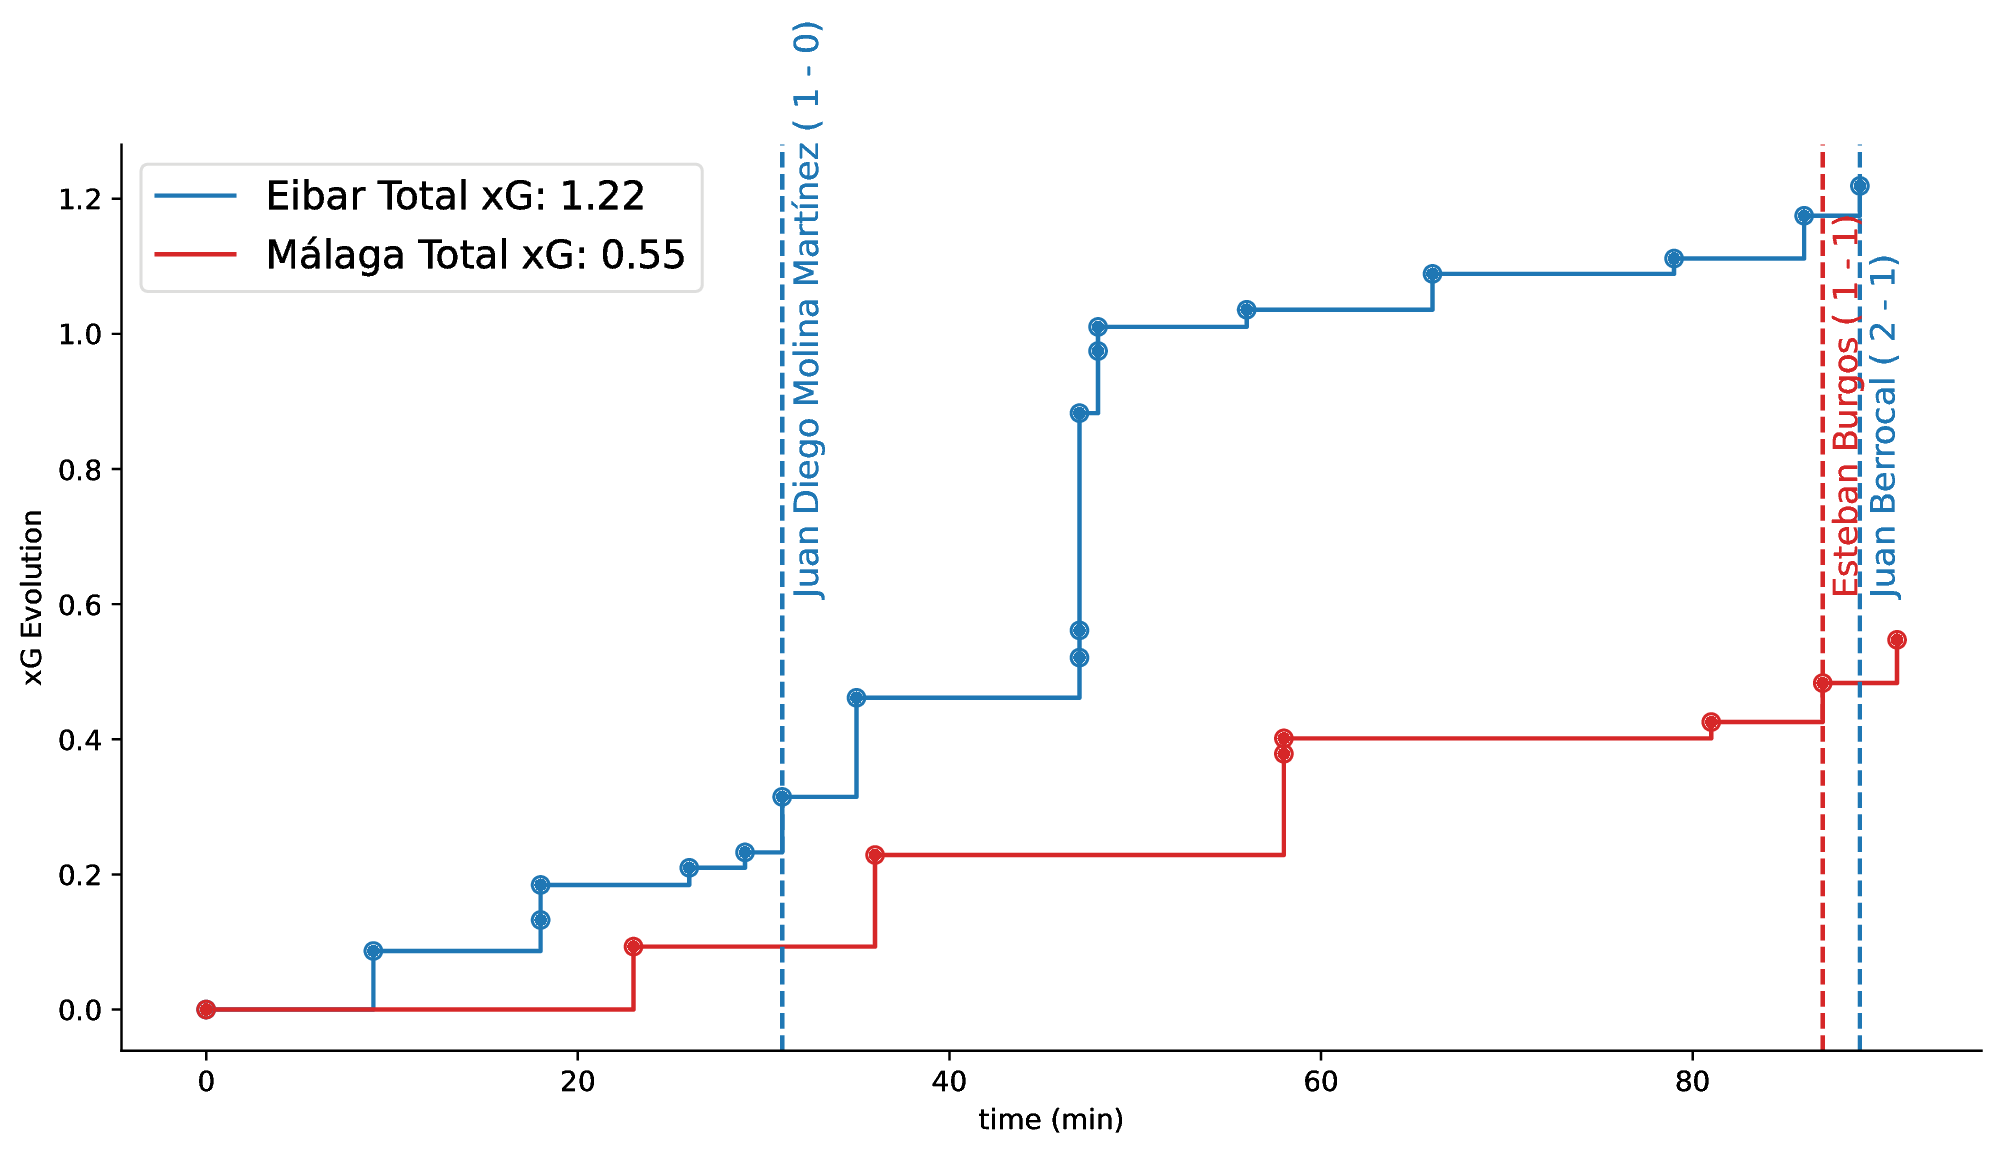
\includegraphics[width=0.8\linewidth,]{imagenes/xg_evol} 

}

\caption{Cumulative development of expected goals (xG) during the Eibar-Malaga match, held on January 15th in Spain’s second division. Each point denotes a shot made by both teams throughout the game. Vertical dashed lines indicate the goal scored, displaying the player and the corresponding score at that specific moment of the match.}\label{fig:xg}
\end{figure}

Expected Goals (xG) have revolutionized the analysis of football by quantifying the quality of scoring opportunities. However, it is important to consider other variables such as player positioning, velocity, passing accuracy, defensive pressure, and tactical formations to gain a broader understanding of the sport. Using the game presented earlier as an example, the next chapter will introduce the broad field of football analytics.

\hypertarget{data-analytics-in-football}{%
\chapter{Data Analytics in football}\label{data-analytics-in-football}}

Looking at an xG evolution figure, such as Fig. \ref{fig:xg}, and solely focusing on shot probabilities while disregarding the spatial distribution of shots and occasions feels like merely scratching the surface of what sport analytics can offer to football.

To illustrate the spatial distribution of shot locations taken by both teams during the game, we can create a shot map for each shot. In Fig. \ref{fig:shotmap}, the size of each data point corresponds to the expected goals (xG) generated for the respective shots, providing insights into the perceived scoring potential. Goals scored are visually highlighted with straight lines, indicating the trajectory the ball followed as it found its way into the opponent's net. Bellow each shot map, a plot of the net can be also found, where goals are represented by football balls, and blocked shots by shadowed points. This detailed analysis not only enhances our understanding of scoring opportunities but also sheds light on the tactical strategies employed by both teams, player positioning, and defensive vulnerabilities. Analyses such as the one above are carried out using the most common
source of data in football: \textbf{Events} datasets.

\begin{figure}[H]

{\centering 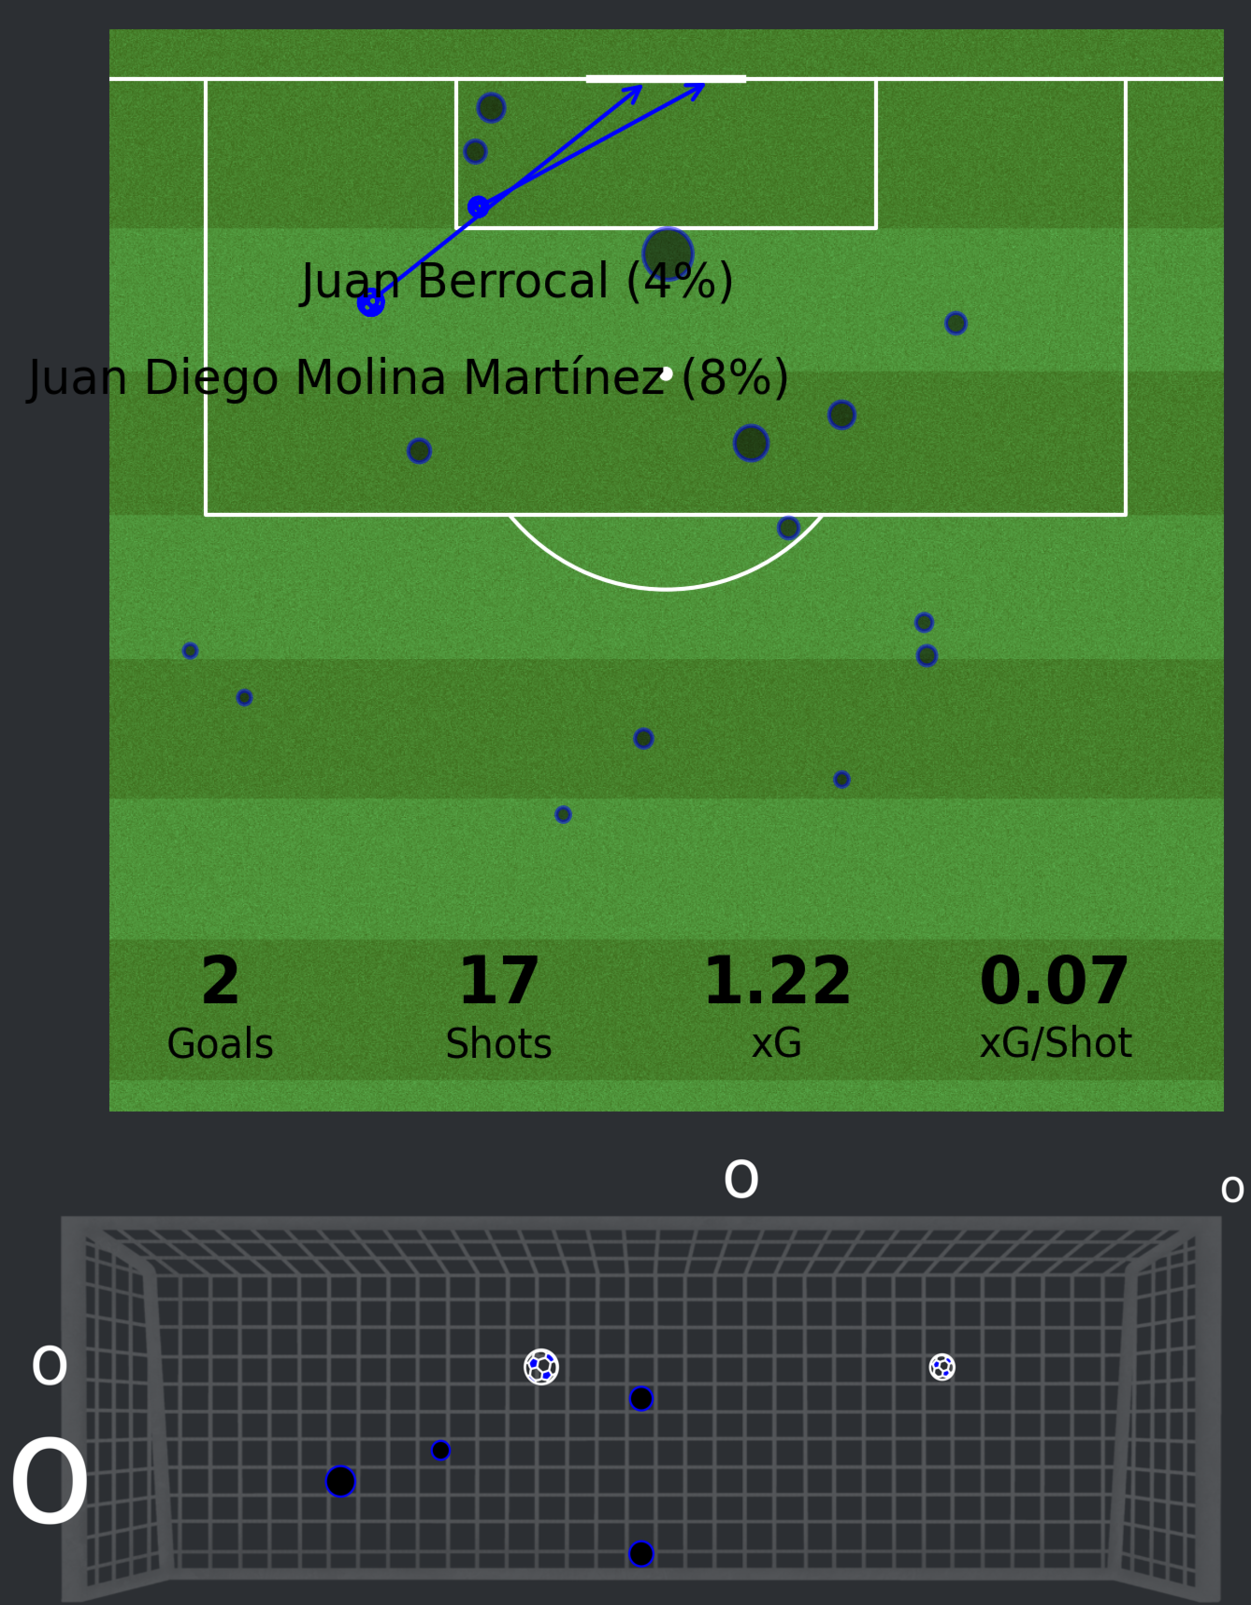
\includegraphics[width=0.45\linewidth,]{imagenes/home_shot_map} 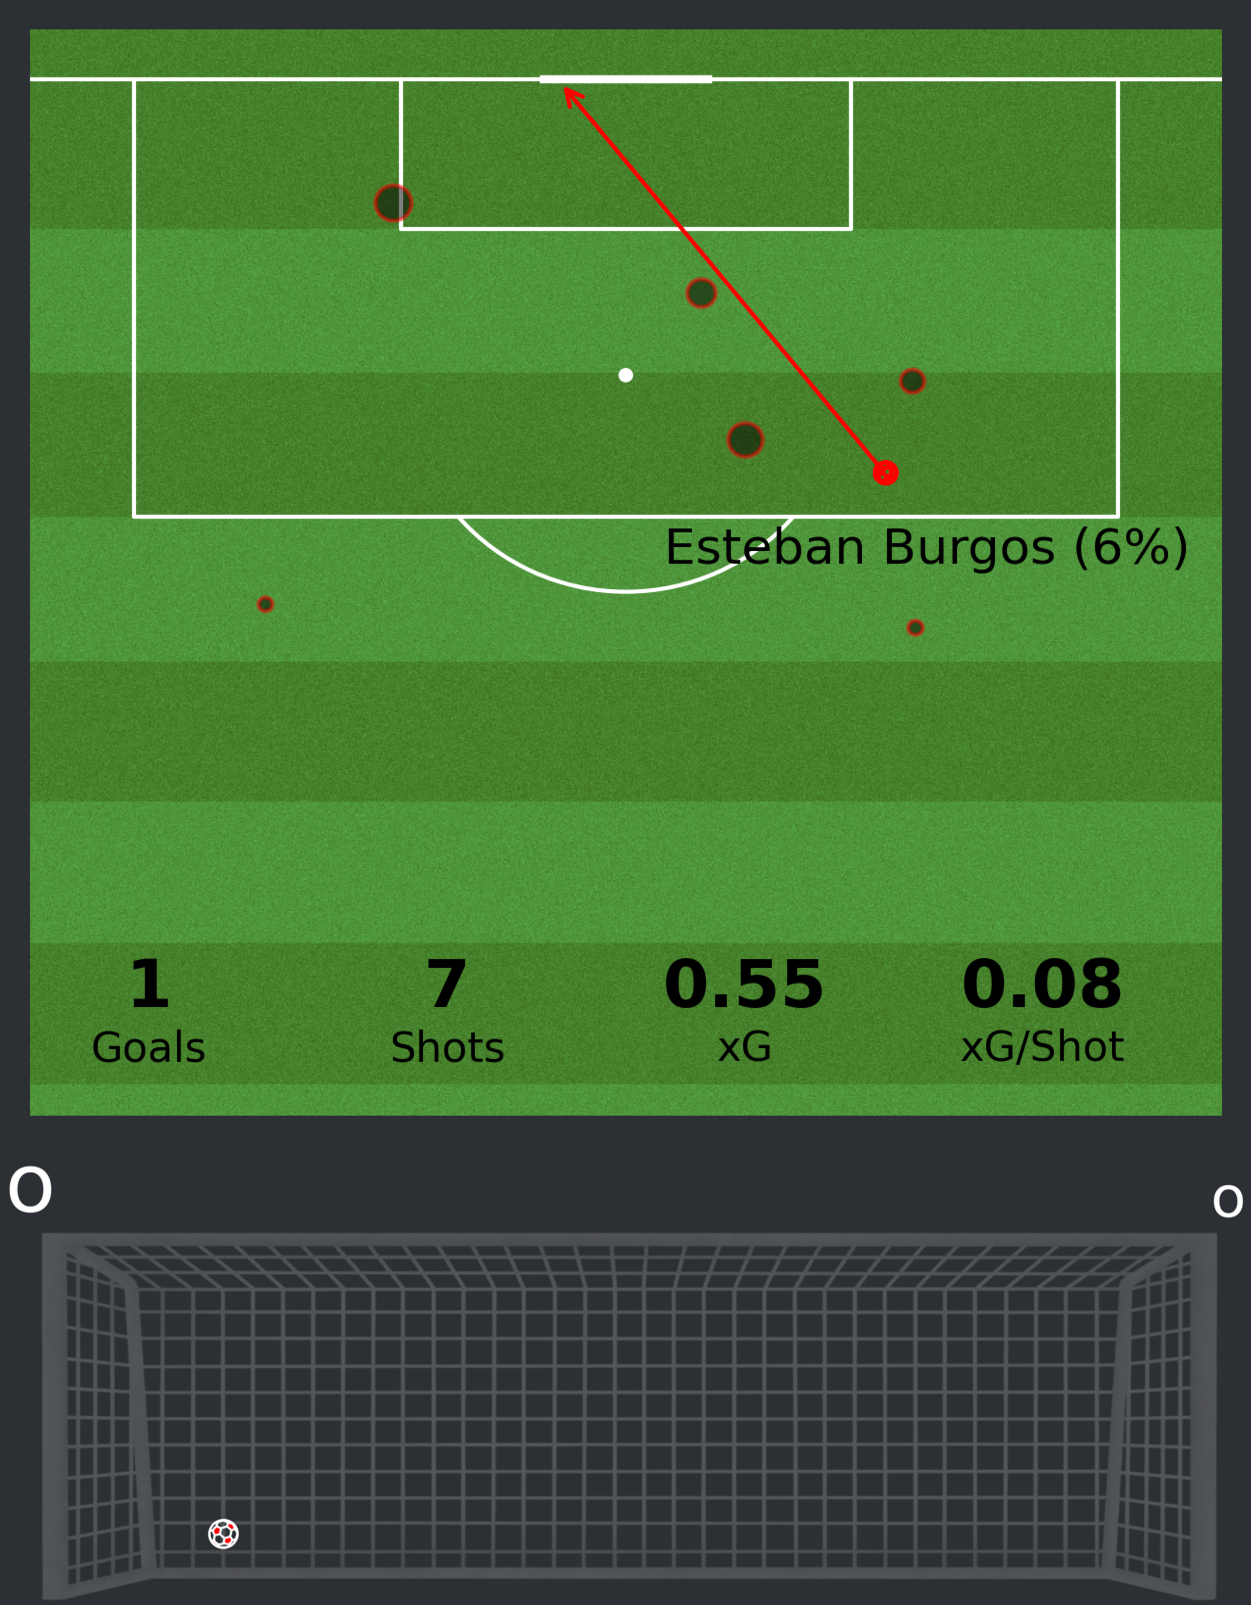
\includegraphics[width=0.45\linewidth,]{imagenes/away_shot_map} 

}

\caption{Shot map of the Eibar (blue, left) - Malaga (red, right) football match. The locations of the points indicate where shots were taken. The size of each point is proportional to the expected goals (xG) generated. Shots that resulted in goals are depicted with a straight line, representing the path the ball took to enter the opponent’s net.}\label{fig:shotmap}
\end{figure}

\hypertarget{events-data}{%
\section{Events data}\label{events-data}}

\texttt{Event\ data} describes specific, human-defined events during a match,
including passes, shots, and fouls. It is captured by human annotators
from various providers. However, this manual process is time-consuming
and typically requires three individuals:

The data collection process is carried out by professional video
analysts (known as operators), who are specialists in football data
collection, using proprietary software (the tagger). The tagger has
undergone several years of development and improvement and is regularly
updated to ensure the highest level of performance is achieved. To
ensure accurate data collection when tagging events in soccer matches,
three operators are assigned: one per team and one supervising the
output of the entire match. This process is based on analysis of the
tagger and soccer match videos. When near-live data delivery is
necessary, a team of four operators may be utilized, with one operator
dedicated to hastening the collection of complex events that require
additional, specific attributes or a quick review \citep{3}.

This type of data structure can be used in a number of ways: it can be
used to measure team performance through general statistics extracted
from event datasets, such as goals, fouls, xG, etc. It can also be used
to create advanced analysis of the team using ensembles of mathematical
tools.

The analysis of the match is furthered through the use of graph theory,
\citep{Buldu}, \citep{NOVILLO2024114355}. Combining
different elements of the events dataset, we can create a graph
corresponding to the passing network of each team, allowing us to
understand the passing structure of both teams.

Figs. \ref{fig:homepass} and \ref{fig:awaypass} illustrate the
passing networks observed in the Eibar versus Málaga football match,
providing insight into the passing interactions and tactical strategies
used by both teams. The nodes in the graphs represent individual players
who participated in the match for each team. The nodes are sized
according to their degree, which represents the amount of ingoing and
outgoing passes. The node position corresponds to the average passing
position of each player. Substitutes are represented by yellow nodes,
and links are created if there have been at least 5 passes made in that
direction between two players. The edge's width corresponds to the
amount of passes made in that direction between the two players.

\begin{figure}[H]

{\centering 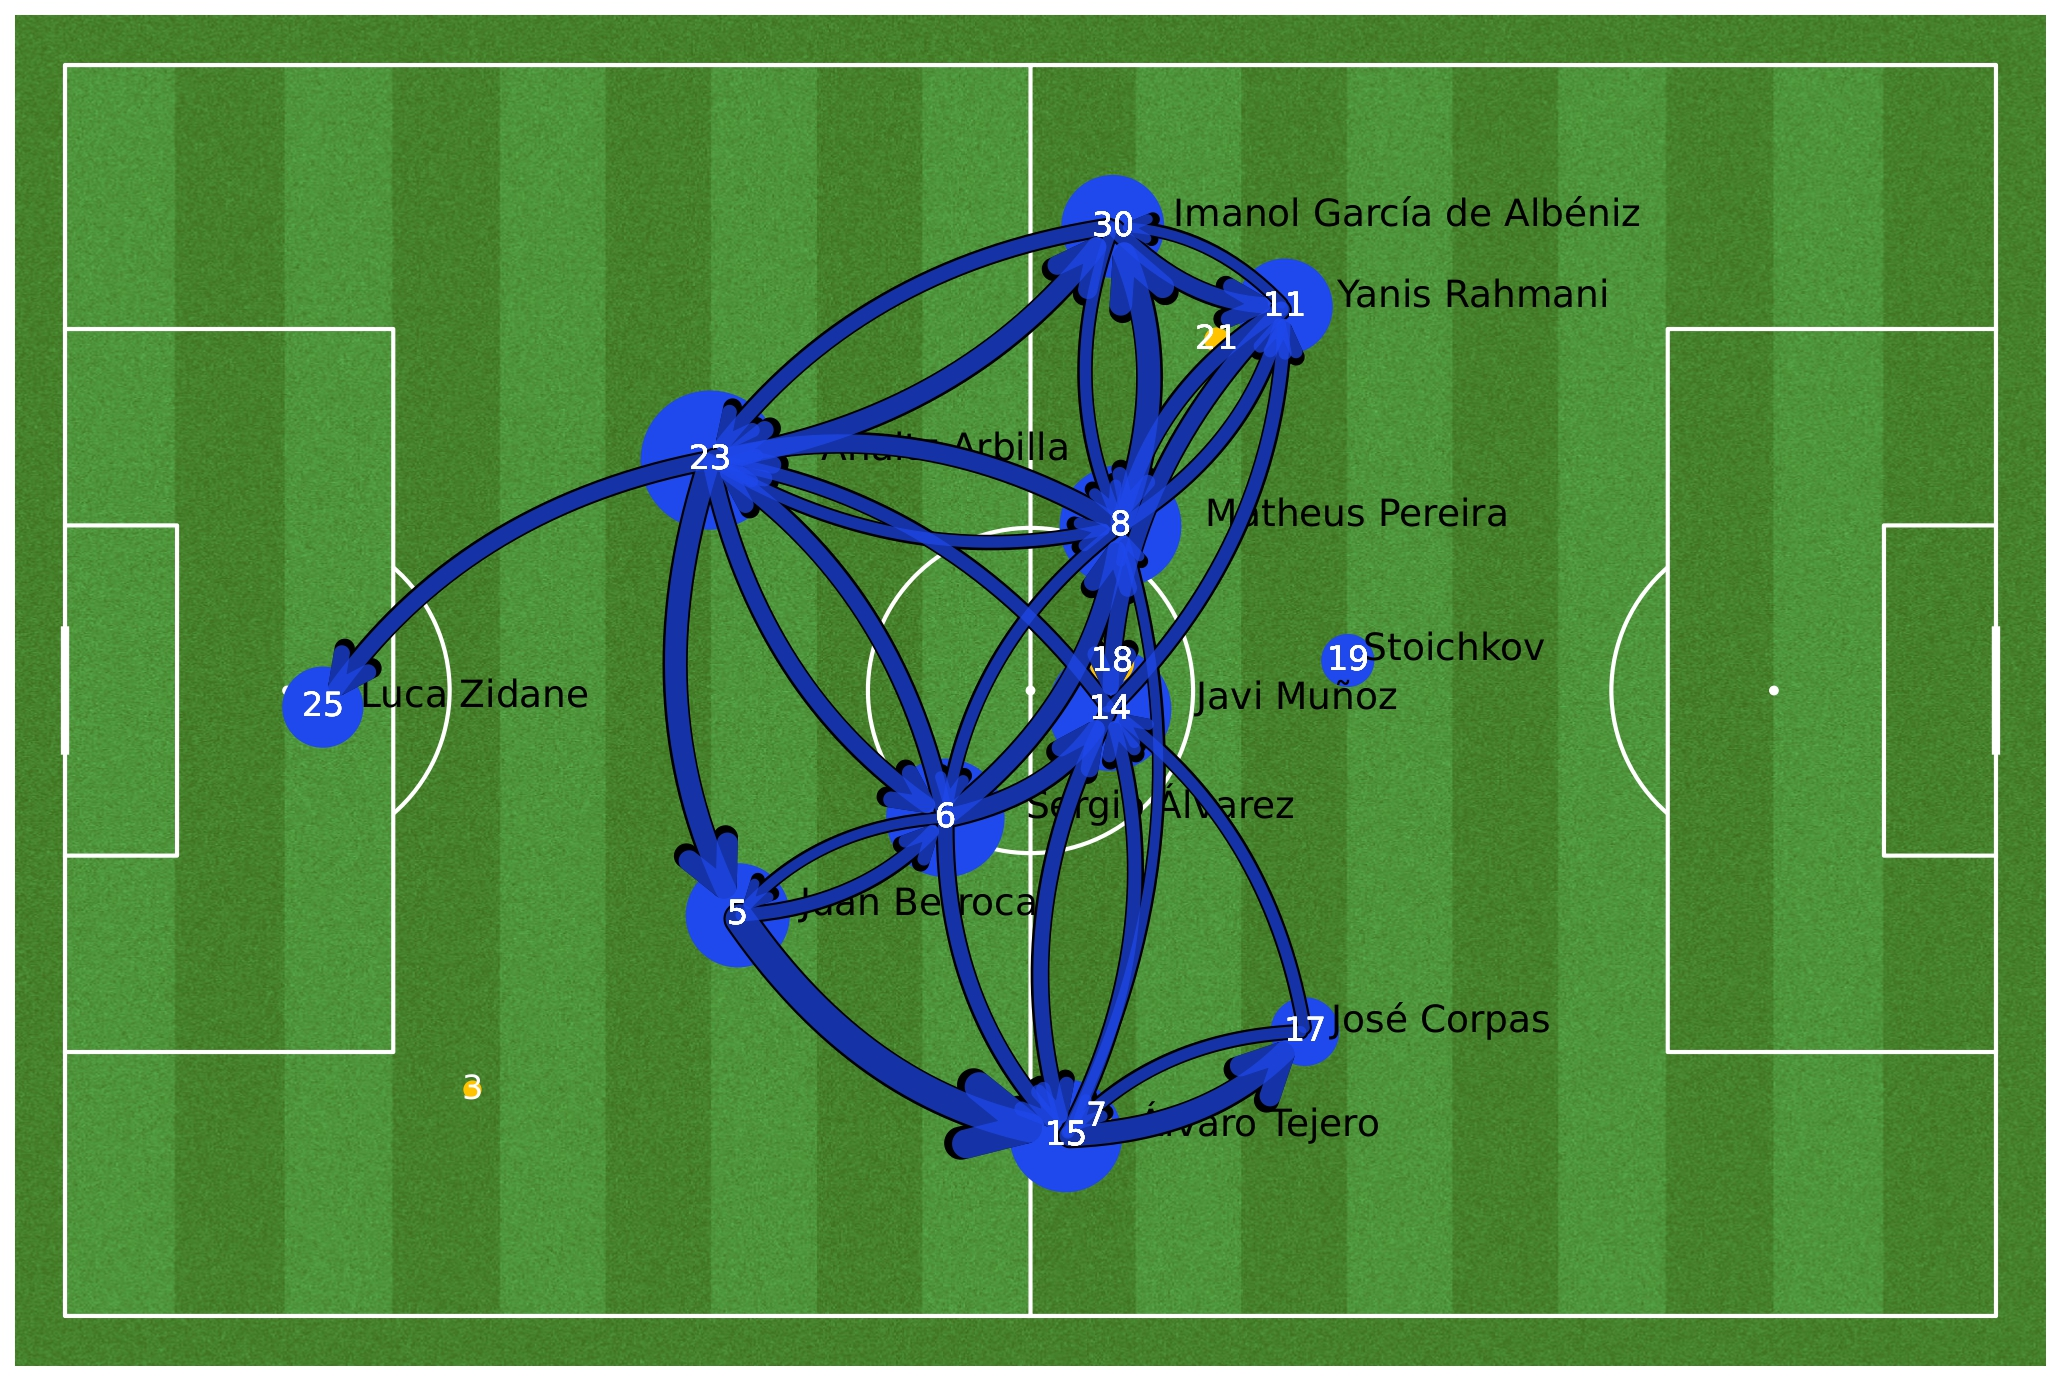
\includegraphics[width=0.8\linewidth,]{imagenes/home_pass_network} 

}

\caption{Representation of the Eibar passing networks of the match Eibar - Málaga. Nodes represent players, edges represent passes between players. The position of the players in the field is their average passing position. The size of the nodes reflects the number of ingoing and outgoing passes (i.e. node’s degree), while the size of the edges is proportional to the number of passes between the players. Substitutes are represented in yellow. A connection is set if those players share at least 5 passes. The edge’s width is proportional to the amount of passes made in that direction between the two players.}\label{fig:homepass}
\end{figure}

\begin{figure}[H]

{\centering 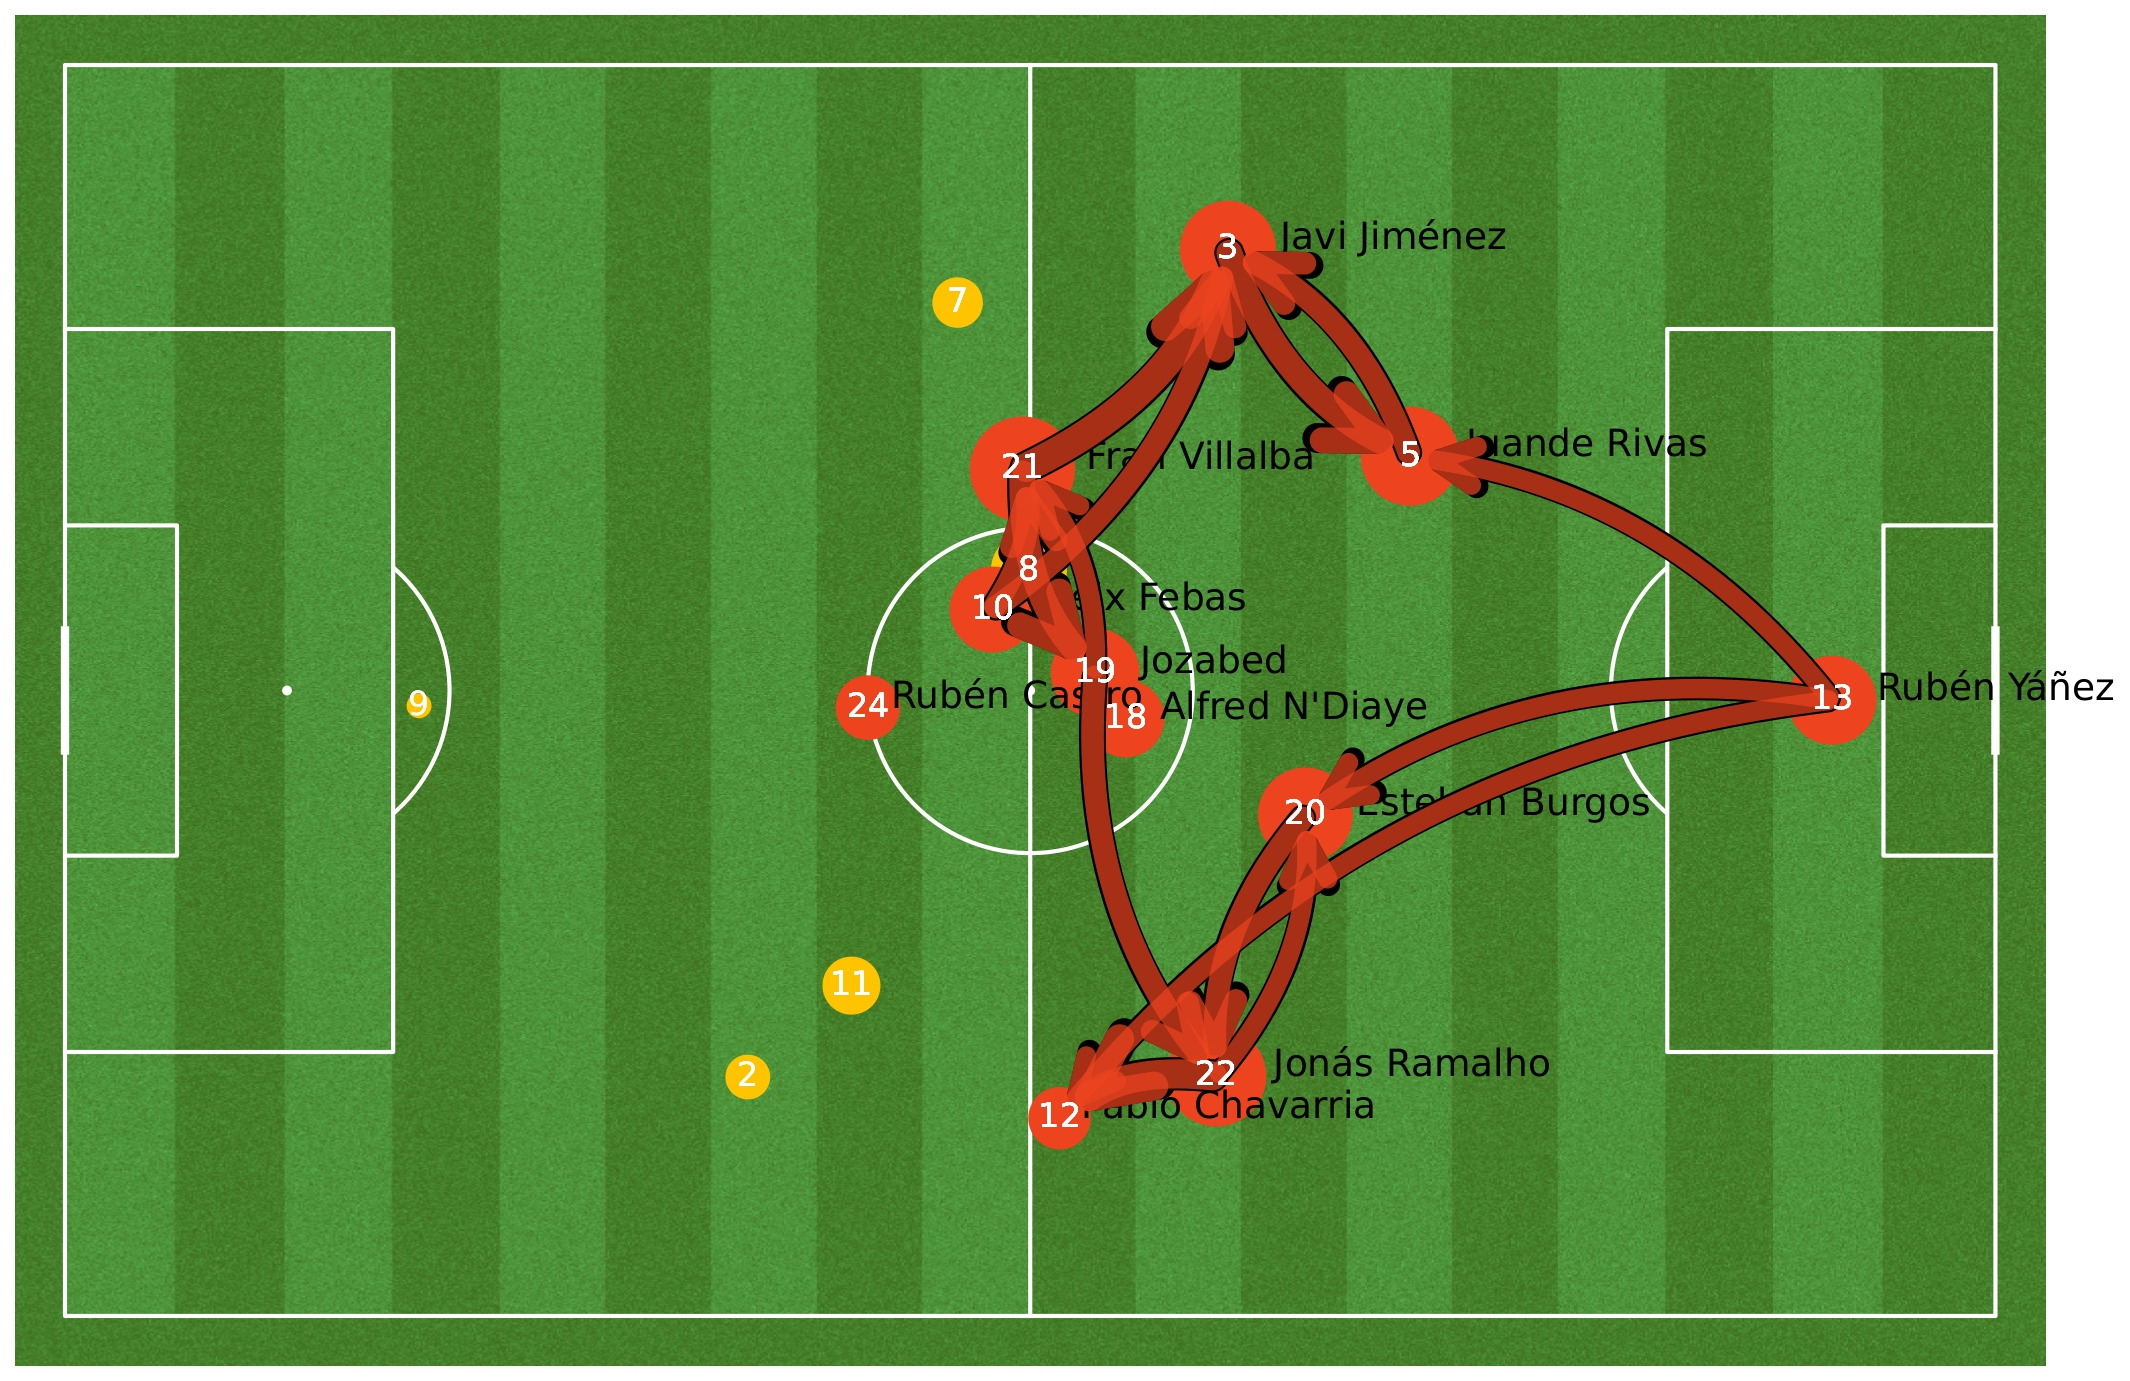
\includegraphics[width=0.8\linewidth,]{imagenes/away_pass_network} 

}

\caption{Representation of the Málaga passing networks of the match Eibar - Málaga. Nodes represent players, edges represent passes between players. The position of the players in the field is their average passing position. The size of the nodes reflects the number of ingoing and outgoing passes (i.e. node’s degree), while the size of the edges is proportional to the number of passes between the players. Substitutes are represented in yellow. A connection is set if those players share at least 5 passes. The edge’s width is proportional to the amount of passes made in that direction between the two players.}\label{fig:awaypass}
\end{figure}

Analysis as the former can be conducted \emph{in real-time}\footnote{Opta uses a combination of human annotation, computer vision, and
  AI modelling to offer real-time data at various levels of detail
  based on customer requirements. In our situation, the data feed
  updates itself when an event such as a goal, foul or pass occurs;
  otherwise, it updates every 90 seconds. \citep{opta}} during the
match using appropriate data sources. Additionally, we could examine
Eibar's macro situation during the 2022-2023 season to better comprehend
how this micro-statistics contribute to the overall perception of the
team.

  \bibliography{bibliografia.bib}

\end{document}
